\chapter{मिश्रणों को अलग करना}\label{ch:g3:separating-mixtures}

आँधी-पानी के बाद सड़क के गड्ढों में भरा पानी भूरा होता है: बारिश का
पानी, जिसमें मिट्टी, रेत और पत्तियों के टुकड़े मिले हैं। फिर भी रसोई के
नल से आने वाला पानी स्वच्छ होता है, और वह भी कभी नदी में बहने से पहले
बारिश ही था। गंदले पानी को फिर से साफ़ कैसे किया जाए? मिलाई गई
चीज़ों को अलग किया जा सकता है। यह अध्याय दिखाता है कैसे, एक-एक विधि करके।

\begin{recall}
\omterm{def:g2:mixing-and-dissolving:mix}{मिलाना} यानी अलग-अलग चीज़ों को एक साथ रखना। चीनी या नमक जैसा ठोस पानी
में \omterm{def:g2:mixing-and-dissolving:dissolve}{घुलता} है: वह आँखों से ओझल हो जाता है, और जो स्वच्छ द्रव बनता है
वह विलयन है। घुला हुआ ठोस अब भी वहीं रहता है: पानी सूखने पर ठोस पीछे
रह जाता है। रेत और मिट्टी नहीं \omterm{def:g2:mixing-and-dissolving:dissolve}{घुलतीं}
(\cref{ch:g2:mixing-and-dissolving})।
\end{recall}

\section{हाथ से छाँटना और चालना}

जब मिश्रण के टुकड़े इतने बड़े हों कि दिखें और उठाए जा सकें, तो उन्हें
अलग करने का सबसे आसान तरीका हाथ से छाँटना है: मूसली से किशमिश एक-एक करके
बीनी जा सकती है। जब टुकड़े बहुत ज़्यादा हों, तो छलनी हमारे लिए छँटाई
कर देती है।

\begin{definition}[चालना]\label{def:g3:separating-mixtures:sieve}
\emph{चालना}\index{चालना} यानी छलनी से मिश्रण के टुकड़ों को उनके
आकार के अनुसार अलग करना; छलनी एक जाली या छेदों से भरी एक प्लेट होती है।
छोटे टुकड़े छेदों से नीचे गिर जाते हैं; बड़े टुकड़े छलनी में रह जाते हैं।
\end{definition}

\begin{example}[बजरी और रेत]\label{ex:g3:separating-mixtures:gravel}
एक मिस्त्री बजरी और रेत के मिश्रण को छलनी के ऊपर हिलाता है। बारीक रेत
नीचे गिरकर ढेर बन जाती है; बजरी जाली पर रह जाती है।
\end{example}

\begin{omfigure}
\begin{tikzpicture}[font=\small]
  % the sieve: a mesh bowl
  \fill[pattern=crosshatch, pattern color=black!45] (-1.6,2.6) arc[start angle=180,
    end angle=360, x radius=1.6, y radius=0.7] -- cycle;
  \draw[black!70, line width=0.8pt] (-1.6,2.6) arc[start angle=180, end angle=360,
    x radius=1.6, y radius=0.7];
  \draw[black!70, line width=0.8pt] (-1.75,2.6) -- (1.75,2.6);
  \draw[black!70, line width=1.4pt] (1.75,2.6) -- (3.0,2.85);
  % gravel kept in the sieve
  \foreach \x/\y/\r in {-0.9/2.25/0.17,-0.45/2.12/0.2,0.05/2.08/0.18,0.5/2.13/0.21,
                        0.95/2.28/0.16,-0.2/2.42/0.15,0.3/2.43/0.17}
    \fill[black!45, draw=black!65] (\x,\y) circle (\r);
  % sand falling
  \foreach \x/\y in {-0.4/1.6,0.1/1.4,0.4/1.7,-0.15/1.15,0.25/1.0,-0.5/0.95,0.0/0.75}
    \fill[orange!60!brown] (\x,\y) circle (0.05);
  % the heap of sand in a bowl
  \fill[orange!45!brown!70] (-1.0,0.12) .. controls (-0.5,0.55) and (0.5,0.55)
    .. (1.0,0.12) -- cycle;
  \draw[black!70, line width=0.8pt] (-1.5,0.5) .. controls (-1.3,0) and (1.3,0)
    .. (1.5,0.5);
  \node[anchor=west] at (2.0,2.2) {बजरी छलनी में रह जाती है};
  \node[anchor=west] at (2.0,1.25) {रेत छेदों से गिर जाती है};
  \node[anchor=west] at (2.0,0.3) {रेत का ढेर};
\end{tikzpicture}

{\small बजरी और रेत के मिश्रण को \omterm{def:g3:separating-mixtures:sieve}{चालना}: टुकड़े अपने आकार के अनुसार
छँट जाते हैं।}
\end{omfigure}

\begin{omfigure}
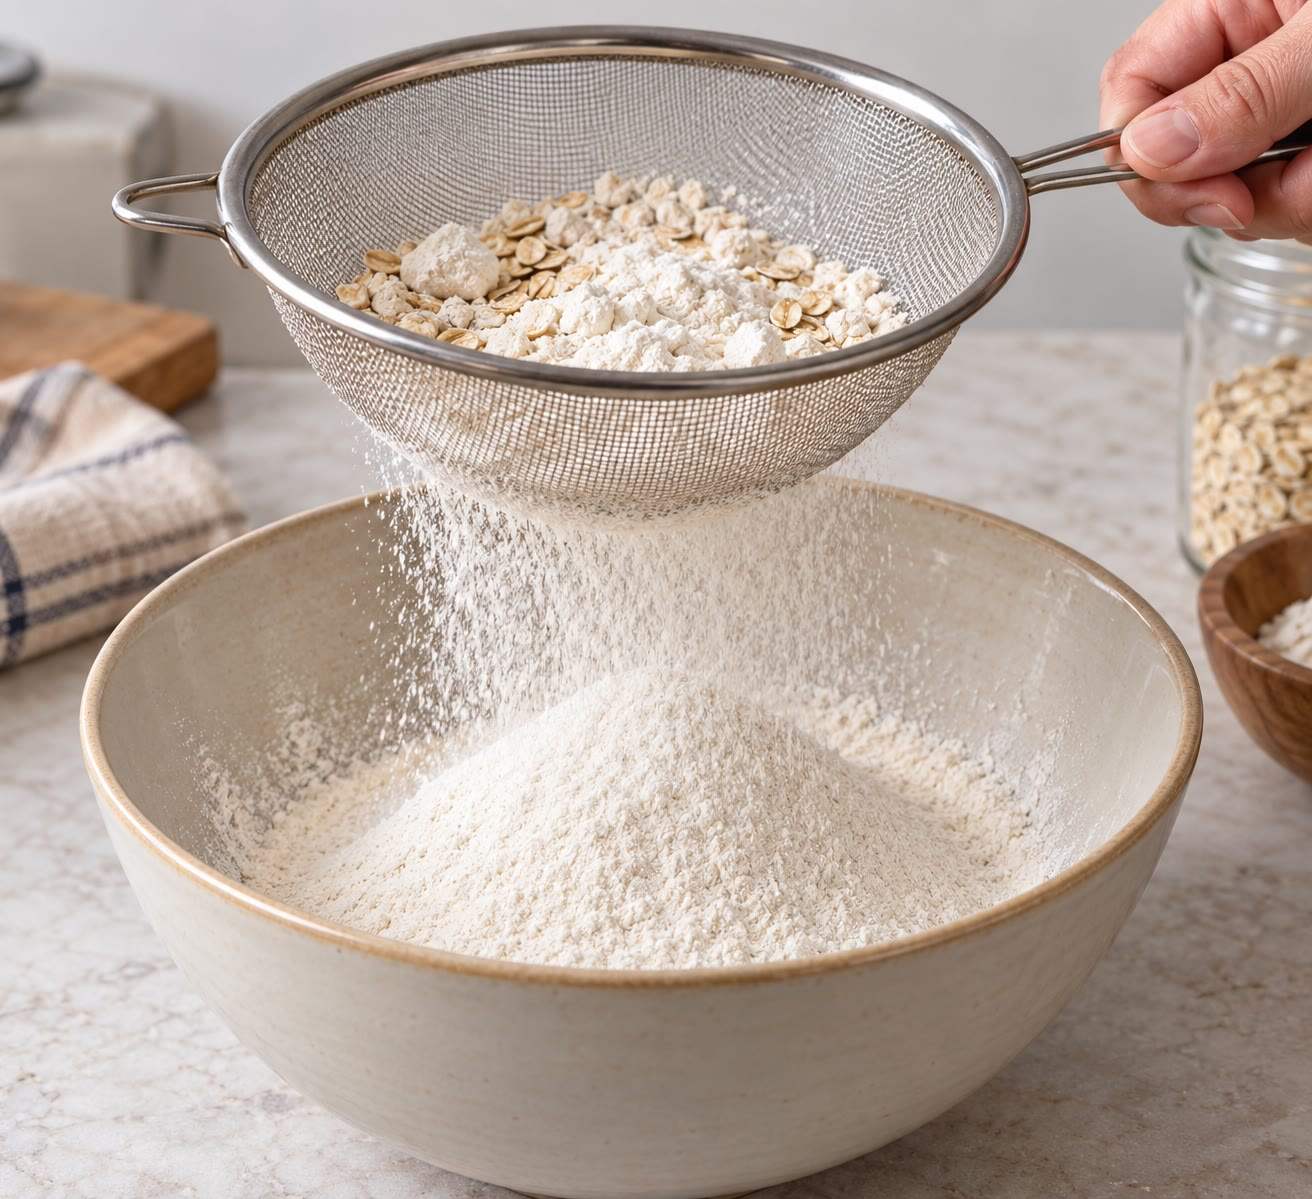
\includegraphics[width=0.55\linewidth]{images/book1/ai/g3-kitchen-sieve.jpg}

{\small रसोई की छलनी: बारीक आटा नीचे निकल जाता है, गाँठें पीछे
रह जाती हैं।}
\end{omfigure}

\section{नीचे बैठने देना और निथारना}

\begin{definition}[अवसादन और निस्तारण]\label{def:g3:separating-mixtures:decant}
पानी और किसी न \omterm{def:g2:mixing-and-dissolving:dissolve}{घुलने} वाले ठोस के मिश्रण को शांत छोड़ा जा सकता है:
ठोस धीरे-धीरे तली में बैठ जाता है। इसे
\emph{अवसादन}\index{अवसादन} कहते हैं। ठोस बैठ जाने पर ऊपर का स्वच्छ
पानी धीरे से दूसरे बर्तन में उँडेला जा सकता है, और ठोस पीछे रह जाता
है: यह \emph{निस्तारण}\index{निस्तारण} है, यानी निथारना।
\end{definition}

\begin{omfigure}
\begin{tikzpicture}[font=\small]
  % 1: stirred, cloudy
  \pic at (0,0) {beaker={0.7}{brown!28}};
  \foreach \x/\y in {-0.5/0.3,-0.2/0.6,0.3/0.4,0.5/0.9,-0.4/1.0,0.1/1.2,0.4/0.15,
                     -0.1/0.25,0.2/0.8,-0.55/0.7}
    \fill[brown!60] (\x,\y) circle (0.03);
  \node[anchor=north, align=center] at (0,-0.15) {चलाने के बाद:\\ धुँधला};
  \draw[->, thick, omProp] (1.1,1.0) -- (2.4,1.0);
  % 2: settled
  \pic at (3.5,0) {beaker={0.7}{omWater!80}};
  \fill[brown!60] (2.7,0) rectangle (4.3,0.25);
  \draw[omGlass, line width=0.7pt] (2.7,0.25) -- (2.7,0) -- (4.3,0) -- (4.3,0.25);
  \node[anchor=north, align=center] at (3.5,-0.15) {शांत छोड़ने पर:\\ मिट्टी नीचे बैठ गई};
  \draw[->, thick, omProp] (4.6,1.0) -- (5.9,1.0);
  % 3: decanted
  \pic at (7.0,0) {beaker={0.1}{omWater!80}};
  \fill[brown!60] (6.2,0) rectangle (7.8,0.25);
  \draw[omGlass, line width=0.7pt] (6.2,0.25) -- (6.2,0) -- (7.8,0) -- (7.8,0.25);
  \pic at (9.2,0) {beaker={0.58}{omWater!80}};
  \node[anchor=north, align=center] at (8.1,-0.15) {निथारने पर: दाईं ओर स्वच्छ\\ पानी, मिट्टी पीछे रही};
\end{tikzpicture}

{\small मिट्टी और पानी के मिश्रण का \omterm{def:g3:separating-mixtures:decant}{अवसादन}, फिर \omterm{def:g3:separating-mixtures:decant}{निस्तारण}।}
\end{omfigure}

\begin{remark}[नीचे बैठने में समय लगता है]\label{rem:g3:separating-mixtures:time}
बड़े, भारी कण कुछ ही मिनटों में बैठ जाते हैं; बहुत बारीक चिकनी मिट्टी में
एक दिन या उससे ज़्यादा लग सकता है, और तब तक पानी थोड़ा धुँधला रहता है।
निथारने से हर कण कभी नहीं हटता: थोड़ा धुँधलापन पानी के साथ उँडेल दिया जाता है।
\end{remark}

\section{छानना}

\begin{definition}[छानना और निस्यंद]\label{def:g3:separating-mixtures:filter}
\emph{छानना}\index{छानना} यानी मिश्रण को किसी छन्ने में से उँडेलना:
कागज़ का पन्ना, कपड़ा या रेत की परत, जिनके छेद इतने छोटे होते हैं कि
ठोस टुकड़े उनसे नहीं निकल पाते। ठोस छन्ने पर रह जाता है; जो स्वच्छ
द्रव छनकर निकलता है, उसे
\emph{निस्यंद}\index{निस्यंद} कहते हैं।
\end{definition}

\begin{omfigure}
\begin{tikzpicture}[font=\small, scale=1.4]
  \pic[transform shape] at (0,0) {beaker={0.35}{omWater!80}};
  \pic[transform shape] at (0,1.4) {funnel={brown!55}};
  % muddy water waiting in the paper cone, above the soil
  \fill[brown!25] (-0.411,2.45) -- (0.411,2.45) -- (0.722,2.8) -- (-0.722,2.8) -- cycle;
  % drops of filtrate
  \foreach \y in {1.15,0.95} \fill[omDef!50] (0,\y) circle (0.04);
  \draw[<-, omProp, thick] (0.75,2.6) -- (2.0,2.9) node[right, text=black]
    {कीप में फ़िल्टर पेपर};
  \draw[<-, omProp, thick] (0.25,2.15) -- (2.0,2.2) node[right, text=black]
    {मिट्टी पेपर पर रह जाती है};
  \draw[<-, omProp, thick] (0.85,0.4) -- (2.0,0.6) node[right, text=black]
    {निस्यंद: स्वच्छ पानी};
\end{tikzpicture}

{\small गंदले पानी को कागज़ के फ़िल्टर से \omterm{def:g3:separating-mixtures:filter}{छानना}।}
\end{omfigure}

\begin{inthelab}[गंदले पानी को छानना]
शिक्षक फ़िल्टर पेपर के एक गोल पन्ने को मोड़कर शंकु बनाते हैं और उसे एक
बीकर के ऊपर रखी काँच की कीप में बिठाते हैं। गंदला पानी शंकु में थोड़ा-थोड़ा
करके डाला जाता है, पेपर के किनारे से ऊपर कभी नहीं। स्वच्छ पानी बूँद-बूँद
बीकर में टपकता है; मिट्टी पेपर पर भूरी परत बना देती है। अगर \omterm{def:g3:separating-mixtures:filter}{निस्यंद}
धुँधला हो, तो या तो पेपर फट गया है या पानी उसके किनारे के ऊपर से निकल गया।
\end{inthelab}

\begin{proposition}[छन्ना घुली हुई चीज़ को नहीं रोकता]\label{prop:g3:separating-mixtures:dissolved}
छन्ना उन ठोस टुकड़ों को रोक लेता है जो घुले नहीं हैं। जो घुला हुआ है,
उसे वह नहीं रोकता: नमकीन पानी छन्ने से निकलकर उतना ही नमकीन रहता है,
और मीठी चाय उतनी ही मीठी।
\end{proposition}

\begin{omfigure}
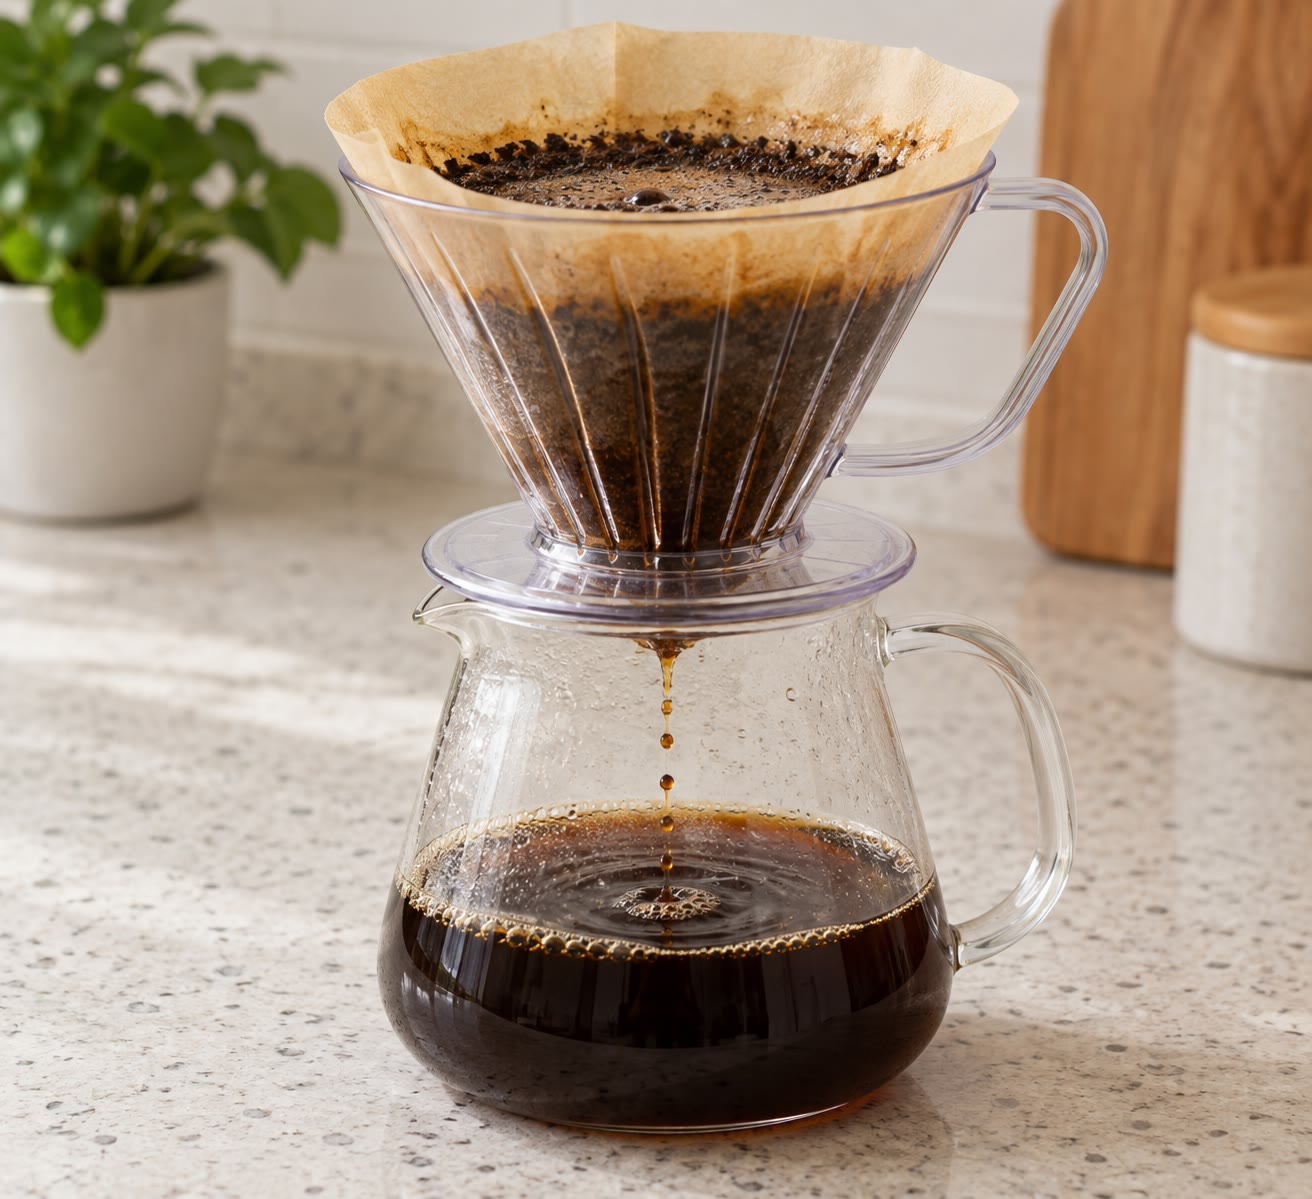
\includegraphics[width=0.5\linewidth]{images/book1/ai/g3-coffee-filter.jpg}

{\small कॉफ़ी बनाना \omterm{def:g3:separating-mixtures:filter}{छानना} ही है: पिसी कॉफ़ी कागज़ में रह जाती है, और
कॉफ़ी \omterm{def:g3:separating-mixtures:filter}{निस्यंद} है।}
\end{omfigure}

\section{पानी को भाप बनाकर उड़ाना}

\begin{definition}[वाष्पन]\label{def:g3:separating-mixtures:evaporate}
पानी में घुले किसी ठोस को वापस पाने के लिए पानी को धूप में या हल्की
आँच पर सूख जाने दिया जाता है: यह
\emph{वाष्पन}\index{वाष्पन} है। पानी हवा में चला जाता है; ठोस
प्याली में रह जाता है।
\end{definition}

\begin{example}[नमकीन पानी से नमक]\label{ex:g3:separating-mixtures:salt}
थोड़ा-सा नमकीन पानी एक उथली प्याली में डालकर धूप वाली खिड़की पर छोड़ दिया
जाता है। कुछ दिन बाद पानी बिल्कुल नहीं बचता, बस नमक की एक सफ़ेद पपड़ी
रहती है: वही नमक जो घुला हुआ था।
\end{example}

\begin{omfigure}
\begin{tikzpicture}[font=\small, scale=1.4]
  \pic[transform shape] at (0,0) {hotplate};
  \pic[transform shape] at (0,0) {evapdish={omWater!80}};
  \node[anchor=north, align=center] at (0,-0.6) {नमकीन पानी,\\ हल्का गरम};
  \draw[->, thick, omProp] (1.5,0.3) -- (3.0,0.3) node[midway, above, text=black]
    {बाद में};
  \pic[transform shape] at (4.5,0) {hotplate};
  \pic[transform shape] at (4.5,0) {evapdish={white!85!black}};
  \foreach \x in {-0.45,-0.25,-0.05,0.15,0.35}
    \fill[white, draw=black!45, line width=0.2pt] (4.5+\x,0.12) rectangle ++(0.09,0.06);
  \node[anchor=north, align=center] at (4.5,-0.6) {पानी नहीं बचा:\\ नमक के क्रिस्टल};
  \foreach \x in {-0.3,0,0.3} \draw[->, black!45, decorate,
    decoration={snake, amplitude=0.6pt, segment length=4pt}] (\x,0.7) -- (\x,1.4);
  \node[anchor=south] at (0,1.4) {पानी हवा में जाता है};
\end{tikzpicture}

{\small प्रयोगशाला में \omterm{def:g3:separating-mixtures:evaporate}{वाष्पन}: शिक्षक प्याली को हॉटप्लेट पर हल्का गरम
करते हैं। नमक प्याली में रह जाता है।}
\end{omfigure}

\section{किस मिश्रण के लिए कौन-सी विधि?}

\begin{method}[अलग करने की विधि चुनना]\label{met:g3:separating-mixtures:choose}
किसी मिश्रण को अलग करने के लिए पूछो:
\begin{enumerate}
  \item क्या टुकड़े बड़े हैं और अलग-अलग आकार के हैं? हाथ से छाँटो, या
        चालो।
  \item क्या किसी द्रव में कोई न \omterm{def:g2:mixing-and-dissolving:dissolve}{घुलने} वाला ठोस है? उसे नीचे बैठने दो और
        निथारो, या ज़्यादा स्वच्छ पानी के लिए छानो।
  \item क्या द्रव में कोई ठोस घुला है? द्रव का \omterm{def:g3:separating-mixtures:evaporate}{वाष्पन} करो:
        ठोस बच जाता है।
\end{enumerate}
अक्सर कई चरण, एक के बाद एक, ज़रूरी होते हैं।
\end{method}

\begin{example}[रेत, नमक और पानी]\label{ex:g3:separating-mixtures:three}
एक मर्तबान में पानी है, जिसमें रेत और नमक हैं। नमक घुल गया है; रेत
नहीं घुली।
\begin{enumerate}
  \item छानो: रेत पेपर पर रह जाती है।
  \item \omterm{def:g3:separating-mixtures:filter}{निस्यंद} स्वच्छ है, पर वह नमकीन पानी है। उसका \omterm{def:g3:separating-mixtures:evaporate}{वाष्पन} करो:
        नमक प्याली में रह जाता है।
\end{enumerate}
दो विधियाँ, एक के बाद एक, रेत और नमक दोनों वापस दे देती हैं।
\end{example}

\begin{example}[नदी से साफ़ पानी]\label{ex:g3:separating-mixtures:plant}
जल-शोधन संयंत्र नदी के पानी को कई चरणों में पीने लायक बनाता है:
\begin{enumerate}
  \item नदी का पानी जालियों से गुज़रता है --- बड़ी-बड़ी झंझरियाँ, जो
        टहनियों, पत्तियों और प्लास्टिक को रोक लेती हैं: यह एक तरह का \omterm{def:g3:separating-mixtures:sieve}{चालना} है;
  \item वह बड़ी-बड़ी टंकियों में ठहरता है, जहाँ कीचड़ तली में बैठ जाता है;
  \item उसे रेत की मोटी परतों से छाना जाता है, जो सबसे बारीक कणों को
        रोक लेती हैं;
  \item कीटाणुओं को मारने वाली किसी चीज़ की बहुत थोड़ी-सी मात्रा मिलाई
        जाती है, ताकि पाइपों में पानी सुरक्षित बना रहे।
\end{enumerate}
\end{example}

\begin{omfigure}
\begin{tikzpicture}[font=\small, node distance=0.45cm,
    box/.style={draw=omDef, fill=omDef!6, rounded corners=2pt, align=center,
      minimum height=1.15cm, text width=2.0cm}]
  \node[box] (r) {नदी का\\ पानी};
  \node[box, right=of r] (s) {जालियाँ\\ (चालना)};
  \node[box, right=of s] (t) {अवसादन\\ टंकियाँ};
  \node[box, right=of t] (f) {रेत के\\ छन्ने};
  \node[box, right=of f] (g) {कीटाणु\\ नष्ट};
  \foreach \a/\b in {r/s,s/t,t/f,f/g} \draw[->, thick, omProp] (\a) -- (\b);
  \node[below=0.15cm of s, font=\footnotesize, align=center] {टहनियाँ,\\ प्लास्टिक};
  \node[below=0.15cm of t, font=\footnotesize, align=center] {कीचड़};
  \node[below=0.15cm of f, font=\footnotesize, align=center] {बारीक कण};
  \draw[->, thick, omProp] (g.south) -- ++(0,-0.8) node[below] {नलों तक};
\end{tikzpicture}

{\small जल-शोधन संयंत्र के चरण। हर चरण के नीचे: वह क्या
हटाता है।}
\end{omfigure}

\begin{omfigure}
\begin{minipage}[t]{0.48\linewidth}\centering
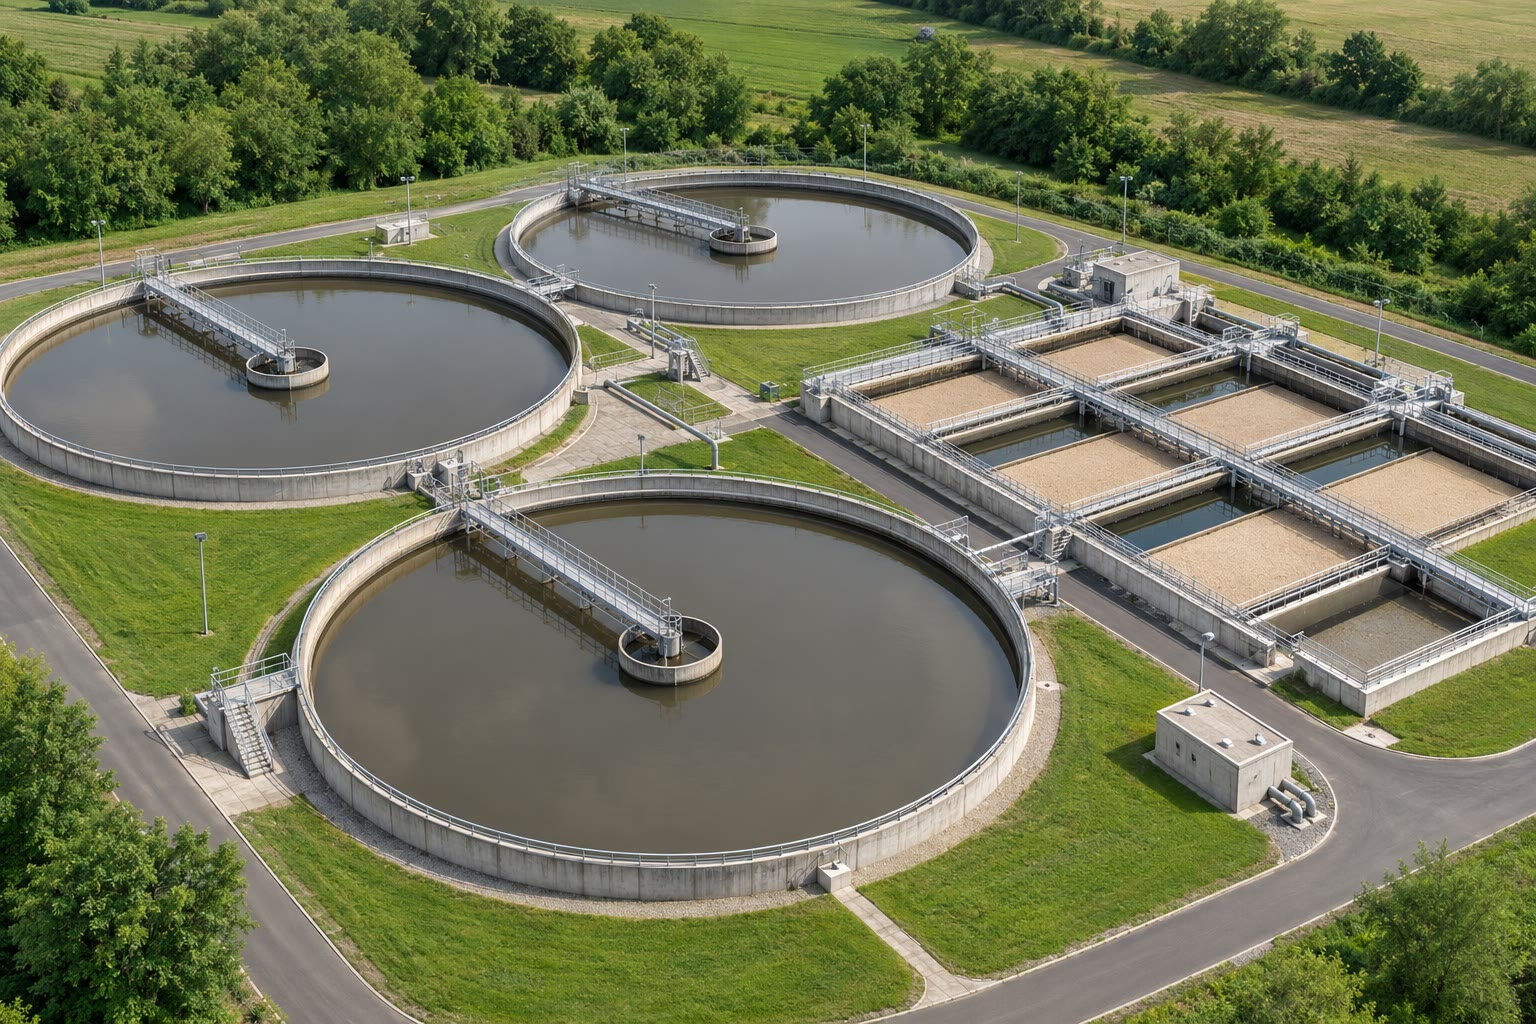
\includegraphics[width=\linewidth,height=4.6cm,keepaspectratio]{images/book1/ai/g3-settling-tanks.jpg}

{\small जल-शोधन संयंत्र की \omterm{def:g3:separating-mixtures:decant}{अवसादन} टंकियाँ।}
\end{minipage}\hfill
\begin{minipage}[t]{0.48\linewidth}\centering
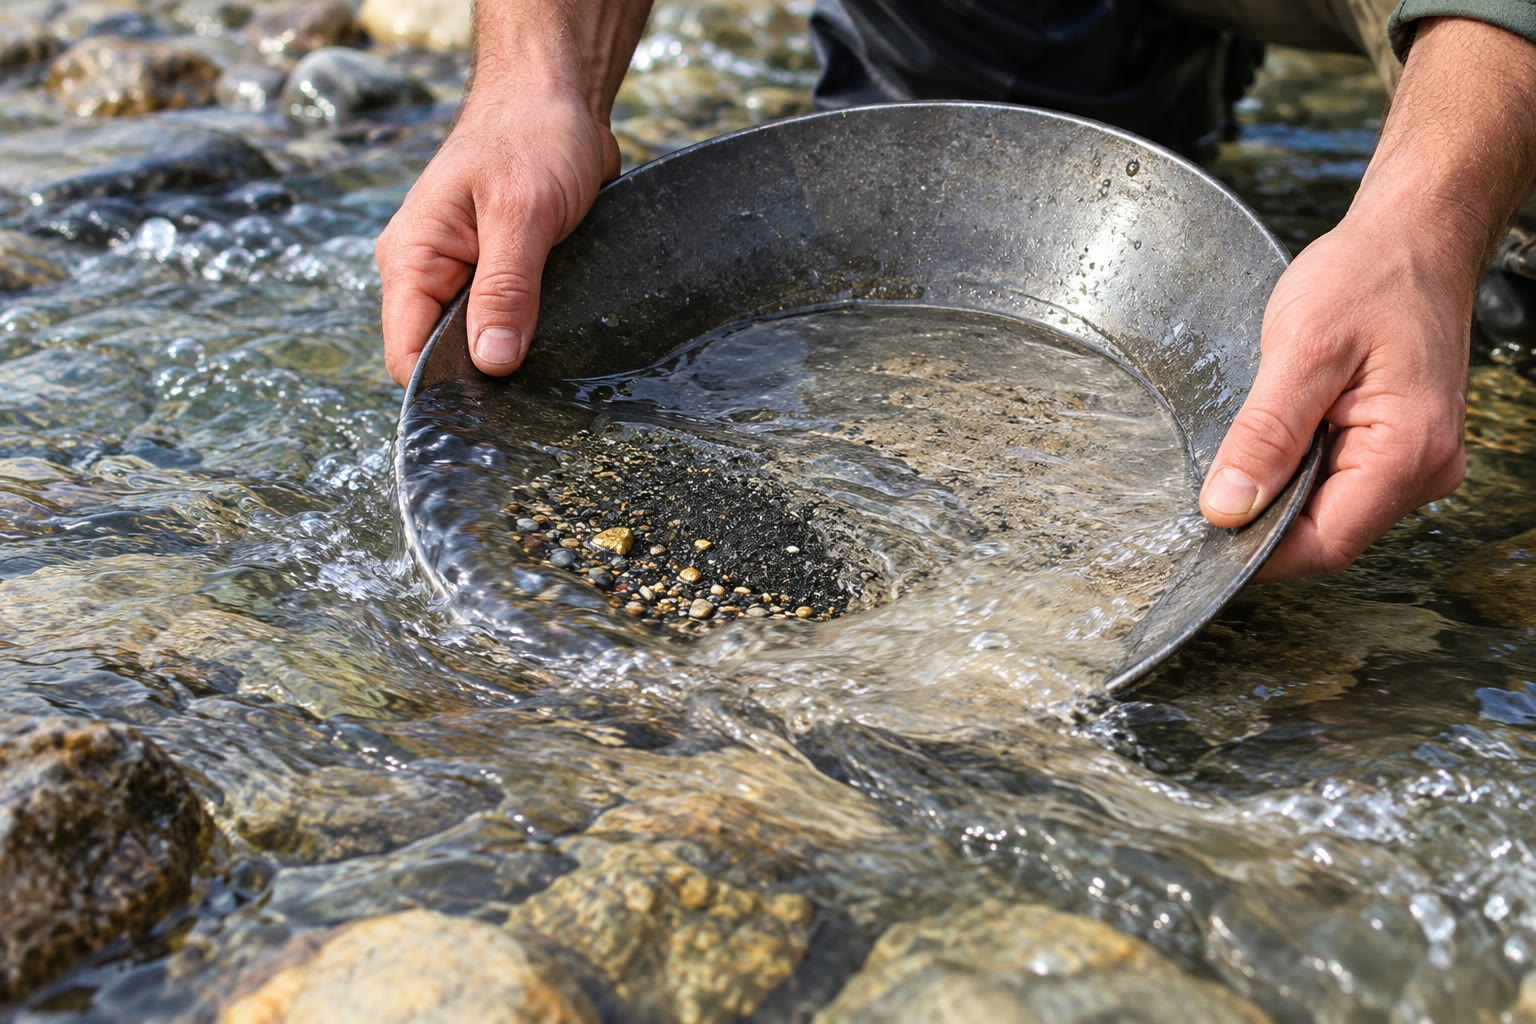
\includegraphics[width=\linewidth,height=4.6cm,keepaspectratio]{images/book1/ai/g3-gold-panning.jpg}

{\small सोना \omterm{def:g3:separating-mixtures:filter}{छानना}: नदी का पानी हल्की रेत को बहा ले जाता है;
भारी कण तसले में रह जाते हैं।}
\end{minipage}
\end{omfigure}

\begin{remark}[स्वच्छ हमेशा साफ़ नहीं होता]\label{rem:g3:separating-mixtures:clean}
छाना हुआ पानी बिल्कुल स्वच्छ दिख सकता है, फिर भी उसमें घुले हुए पदार्थ
और दिखने में बहुत छोटे कीटाणु हो सकते हैं। इसीलिए कोई भी गड्ढे या
नाले का पानी नहीं पीता, छानने के बाद भी नहीं।
\end{remark}

\section{अभ्यास}

\begin{exercise}[$\star$]\label{exo:g3:separating-mixtures:1}
मटर को चावल के दानों से अलग करने के लिए तुम कौन-सी विधि अपनाओगे?
\end{exercise}

\begin{exercise}[$\star$]\label{exo:g3:separating-mixtures:2}
गंदले पानी का एक गिलास एक घंटे के लिए मेज़ पर छोड़ दिया जाता है। मिट्टी
का क्या होता है? इसे क्या कहते हैं?
\end{exercise}

\begin{exercise}[$\star$]\label{exo:g3:separating-mixtures:3}
\omterm{def:g3:separating-mixtures:filter}{निस्यंद} क्या है? कॉफ़ी बनाते समय \omterm{def:g3:separating-mixtures:filter}{निस्यंद} क्या होता है, बताओ।
\end{exercise}

\begin{exercise}[$\star$]\label{exo:g3:separating-mixtures:4}
नमकीन पानी को फ़िल्टर पेपर से उँडेला जाता है। क्या \omterm{def:g3:separating-mixtures:filter}{निस्यंद} नमकीन है?
समझाओ।
\end{exercise}

\begin{exercise}[$\star$]\label{exo:g3:separating-mixtures:5}
चीनी के पानी के एक गिलास से चीनी वापस कैसे पाई जा सकती है?
\end{exercise}

\begin{exercise}[$\star$]\label{exo:g3:separating-mixtures:6}
छलनी वाला चित्र देखो। कौन-से टुकड़े छलनी में रह जाते हैं? बाकी टुकड़े
नीचे क्यों गिर जाते हैं?
\end{exercise}

\begin{exercise}[$\star$]\label{exo:g3:separating-mixtures:7}
हर मिश्रण को एक विधि से मिलाओ --- \omterm{def:g3:separating-mixtures:sieve}{चालना}, \omterm{def:g3:separating-mixtures:filter}{छानना} या \omterm{def:g3:separating-mixtures:evaporate}{वाष्पन}:
(क) रेत और कंकड़; (ख) पानी में खड़िया का चूर्ण; (ग) पानी में नमक।
\end{exercise}

\begin{exercise}[$\star$]\label{exo:g3:separating-mixtures:8}
जल-शोधन संयंत्र वाला चित्र देखो। पानी कितने चरणों से गुज़रता है?
कौन-सा चरण कीचड़ हटाता है?
\end{exercise}

\begin{exercise}[$\star$]\label{exo:g3:separating-mixtures:9}
रेत, नमक और पानी वाले मर्तबान से रेत और नमक वापस पाने के लिए इन चरणों
को सही क्रम में लगाओ: \omterm{def:g3:separating-mixtures:filter}{निस्यंद} का \omterm{def:g3:separating-mixtures:evaporate}{वाष्पन} करो; छानो; पेपर से रेत
इकट्ठा करो।
\end{exercise}

\begin{exercise}[$\star\star$]\label{exo:g3:separating-mixtures:10}
क्या छन्ना समुद्र के पानी को पीने लायक बना सकता है? समझाओ कि क्यों नहीं।
\end{exercise}

\begin{exercise}[$\star\star$]\label{exo:g3:separating-mixtures:11}
चाय से भरी केतली में चाय की पत्तियाँ पड़ी हैं। इस अध्याय में देखी गई
ऐसी दो विधियाँ बताओ जो चाय को पत्तियों से अलग करती हैं।
\end{exercise}
